\documentclass[14pt]{extbook}
\usepackage{multicol, enumerate, enumitem, hyperref, color, soul, setspace, parskip, fancyhdr} %General Packages
\usepackage{amssymb, amsthm, amsmath, latexsym, units, mathtools} %Math Packages
\everymath{\displaystyle} %All math in Display Style
% Packages with additional options
\usepackage[headsep=0.5cm,headheight=12pt, left=1 in,right= 1 in,top= 1 in,bottom= 1 in]{geometry}
\usepackage[usenames,dvipsnames]{xcolor}
\usepackage{dashrule}  % Package to use the command below to create lines between items
\newcommand{\litem}[1]{\item#1\hspace*{-1cm}\rule{\textwidth}{0.4pt}}
\pagestyle{fancy}
\lhead{Progress Quiz 7}
\chead{}
\rhead{Version C}
\lfoot{6523-2736}
\cfoot{}
\rfoot{test}
\begin{document}

\begin{enumerate}
\litem{
Find the equation of the line described below. Write the linear equation as $ y=mx+b $ and choose the intervals that contain $m$ and $b$.\[ \text{Parallel to } 5 x - 3 y = 7 \text{ and passing through the point } (10, 3). \]\begin{enumerate}[label=\Alph*.]
\item \( m \in [0.4, 0.8] \hspace*{3mm} b \in [-13.67, -9.67] \)
\item \( m \in [-3.3, -1] \hspace*{3mm} b \in [18.67, 22.67] \)
\item \( m \in [1.3, 2.6] \hspace*{3mm} b \in [-7, -5] \)
\item \( m \in [1.3, 2.6] \hspace*{3mm} b \in [9.67, 14.67] \)
\item \( m \in [1.3, 2.6] \hspace*{3mm} b \in [-13.67, -9.67] \)

\end{enumerate} }
\litem{
First, find the equation of the line containing the two points below. Then, write the equation as $ y=mx+b $ and choose the intervals that contain $m$ and $b$.\[ (-6, 2) \text{ and } (-5, -9) \]\begin{enumerate}[label=\Alph*.]
\item \( m \in [-12, -8] \hspace*{3mm} b \in [61, 66] \)
\item \( m \in [-12, -8] \hspace*{3mm} b \in [6, 14] \)
\item \( m \in [-12, -8] \hspace*{3mm} b \in [-65, -58] \)
\item \( m \in [-12, -8] \hspace*{3mm} b \in [-6, 0] \)
\item \( m \in [10, 15] \hspace*{3mm} b \in [46, 52] \)

\end{enumerate} }
\litem{
Solve the equation below. Then, choose the interval that contains the solution.\[ -5(-4x + 7) = -16(11x -6) \]\begin{enumerate}[label=\Alph*.]
\item \( x \in [-0.32, -0.24] \)
\item \( x \in [0.24, 0.35] \)
\item \( x \in [0.62, 0.73] \)
\item \( x \in [0.36, 0.5] \)
\item \( \text{There are no real solutions.} \)

\end{enumerate} }
\litem{
Solve the linear equation below. Then, choose the interval that contains the solution.\[ \frac{6x -9}{2} - \frac{9x + 9}{4} = \frac{4x -8}{5} \]\begin{enumerate}[label=\Alph*.]
\item \( x \in [-15, -11] \)
\item \( x \in [-204, -198] \)
\item \( x \in [-104, -99] \)
\item \( x \in [-1.74, 3.26] \)
\item \( \text{There are no real solutions.} \)

\end{enumerate} }
\litem{
Write the equation of the line in the graph below in Standard form $Ax+By=C$. Then, choose the intervals that contain $A, B, \text{ and } C$.
\begin{center}
    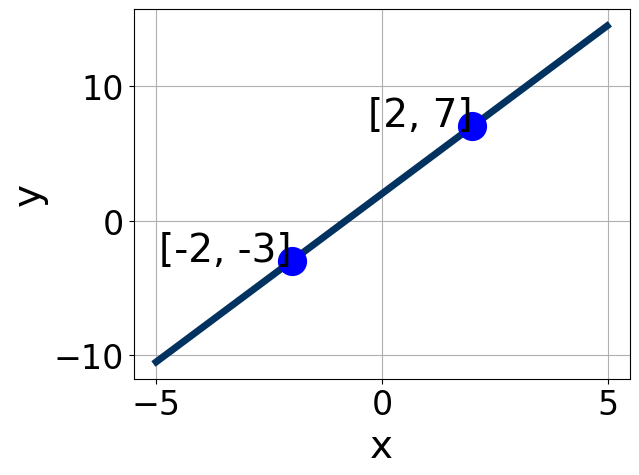
\includegraphics[width=0.5\textwidth]{../Figures/linearGraphToStandardCopyC.png}
\end{center}
\begin{enumerate}[label=\Alph*.]
\item \( A \in [-3.9, 3.7], \hspace{3mm} B \in [-0.5, 2.7], \text{ and } \hspace{3mm} C \in [-0.6, 4.2] \)
\item \( A \in [3.1, 4.7], \hspace{3mm} B \in [-8.2, -3.4], \text{ and } \hspace{3mm} C \in [-6.2, -2.1] \)
\item \( A \in [-3.9, 3.7], \hspace{3mm} B \in [-2.2, -0.5], \text{ and } \hspace{3mm} C \in [-1.7, -0.4] \)
\item \( A \in [3.1, 4.7], \hspace{3mm} B \in [1.3, 6.8], \text{ and } \hspace{3mm} C \in [2.2, 9] \)
\item \( A \in [-4.4, -3.5], \hspace{3mm} B \in [-8.2, -3.4], \text{ and } \hspace{3mm} C \in [-6.2, -2.1] \)

\end{enumerate} }
\litem{
Solve the linear equation below. Then, choose the interval that contains the solution.\[ \frac{5x + 8}{2} - \frac{5x -8}{4} = \frac{3x + 9}{7} \]\begin{enumerate}[label=\Alph*.]
\item \( x \in [-1.9, -0.5] \)
\item \( x \in [0.1, 2.3] \)
\item \( x \in [-10, -7.8] \)
\item \( x \in [-7.2, -2.6] \)
\item \( \text{There are no real solutions.} \)

\end{enumerate} }
\litem{
First, find the equation of the line containing the two points below. Then, write the equation as $ y=mx+b $ and choose the intervals that contain $m$ and $b$.\[ (5, 7) \text{ and } (10, 5) \]\begin{enumerate}[label=\Alph*.]
\item \( m \in [-0.85, 0.34] \hspace*{3mm} b \in [-5.44, -3.99] \)
\item \( m \in [0.28, 1.64] \hspace*{3mm} b \in [0.15, 1.14] \)
\item \( m \in [-0.85, 0.34] \hspace*{3mm} b \in [8.51, 10.71] \)
\item \( m \in [-0.85, 0.34] \hspace*{3mm} b \in [-10.39, -8.81] \)
\item \( m \in [-0.85, 0.34] \hspace*{3mm} b \in [1.7, 2.37] \)

\end{enumerate} }
\litem{
Solve the equation below. Then, choose the interval that contains the solution.\[ -2(10x + 17) = -12(-7x + 16) \]\begin{enumerate}[label=\Alph*.]
\item \( x \in [1.36, 2.01] \)
\item \( x \in [3.4, 3.99] \)
\item \( x \in [-2.73, -1.34] \)
\item \( x \in [1.84, 3.15] \)
\item \( \text{There are no real solutions.} \)

\end{enumerate} }
\litem{
Write the equation of the line in the graph below in Standard form $Ax+By=C$. Then, choose the intervals that contain $A, B, \text{ and } C$.
\begin{center}
    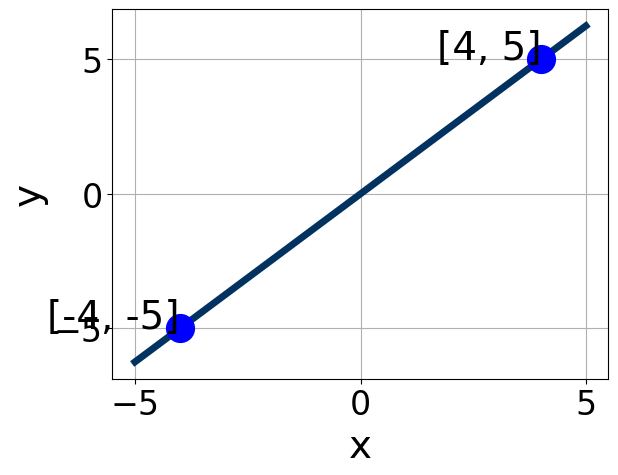
\includegraphics[width=0.5\textwidth]{../Figures/linearGraphToStandardC.png}
\end{center}
\begin{enumerate}[label=\Alph*.]
\item \( A \in [-1.3, -0.9], \hspace{3mm} B \in [0.77, 1.5], \text{ and } \hspace{3mm} C \in [-6, 1] \)
\item \( A \in [4, 5.1], \hspace{3mm} B \in [-4.18, -3.5], \text{ and } \hspace{3mm} C \in [12, 18] \)
\item \( A \in [4, 5.1], \hspace{3mm} B \in [3.18, 5.37], \text{ and } \hspace{3mm} C \in [-12, -11] \)
\item \( A \in [-1.3, -0.9], \hspace{3mm} B \in [-1.24, -0.3], \text{ and } \hspace{3mm} C \in [-2, 8] \)
\item \( A \in [-5.7, -3.8], \hspace{3mm} B \in [3.18, 5.37], \text{ and } \hspace{3mm} C \in [-12, -11] \)

\end{enumerate} }
\litem{
Find the equation of the line described below. Write the linear equation as $ y=mx+b $ and choose the intervals that contain $m$ and $b$.\[ \text{Parallel to } 4 x - 5 y = 4 \text{ and passing through the point } (-8, -6). \]\begin{enumerate}[label=\Alph*.]
\item \( m \in [-0.91, -0.3] \hspace*{3mm} b \in [-12.59, -11.76] \)
\item \( m \in [1.02, 1.66] \hspace*{3mm} b \in [-0.14, 1.11] \)
\item \( m \in [0.02, 1.17] \hspace*{3mm} b \in [-0.7, -0.25] \)
\item \( m \in [0.02, 1.17] \hspace*{3mm} b \in [1.2, 2.63] \)
\item \( m \in [0.02, 1.17] \hspace*{3mm} b \in [-0.14, 1.11] \)

\end{enumerate} }
\end{enumerate}

\end{document}